\documentclass[a4paper,12pt]{article}

\usepackage[dutch]{babel}
\usepackage{fancyhdr}
\usepackage{graphicx}
\usepackage[pdftex,bookmarks=true]{hyperref}
\usepackage[utf8]{inputenc}
\usepackage{fullpage}
\usepackage{parskip}
\usepackage{float}
\usepackage{subcaption}
\usepackage{listings}

\title{Samenvatting Databanken II \\ \large TIN 2 - HoGent}
\author{Lorenz Verschingel}

\begin{document}
\maketitle

\section{SQL}

\subsection{Inner join}
Voorbeeld van een inner join:
\begin{lstlisting}[language=sql]
SELECT au_lastName, au_FirstName, title_id
FROM authors
JOIN titleAuthor ON authors.au_id = titleauthor.au_id
\end{lstlisting}
Hier worden alle records van authors en titleAuthor aan elkaar gekoppeld op basis van au\_id.

\subsection{Aliassen}
Het gebruik van tabel aliassen gebeurt via het keyword 'AS' of door een spatie.

\begin{lstlisting}[language=sql]
SELECT au_lname, au_fname, title_id
FROM authors AS A
JOIN titleauthor TA ON A.au_id = TA.au_id
\end{lstlisting}

\subsection{Inner join van meerdere tabellen}
Gegevens kunnen ook over meerdere tabellen verspreid zitten. Hierbij moeten dan meerdere tabellen aan elkaar gekoppeld worden.
\begin{lstlisting}[language=sql]
SELECT au_lname, au_fname, title
FROM authors A
JOIN titleauthor TA ON A.au_id= TA.au_id
JOIN titles T ON TA.title_id= T.title_id
\end{lstlisting}
Het kan zijn dat er enkel gegevens uit 2 tabellen worden getoond, maar dat er in werkelijkheid meerdere tabellen gekoppeld zijn omdat het geen directe koppeling is tussen de tabellen waaruit de gegevens komen.

\subsection{Outer join}
Een outer join retourneert alle records van 1 tabel, zelfs als er geen gerelateerd record bestaat in de andere tabel.

Er zijn 3 types van outer join:
\begin{enumerate}
\item Left outer join retourneert alle rijen van de eerst genoemde tabel in de FROM clause.

In sql is dit de LEFT JOIN
\item Right outer join retourneert alle rijen van de tweede genoemde tabel in de FROM clause.

In sql is dit de RIGHT JOIN
\item Full outer join retourneert ook rijen uit de eerste en tweede tabel die geen corresponderende entry hebben in de andere tabel.

In sql is dit de CROSS JOIN
\end{enumerate}

\subsection{Union}
Via een UNION combineer je het resultaat van 2 of meerdere queriesin 1 resultaattabel.
\begin{lstlisting}[language=sql]
SELECT ... FROM ... WHERE ...
UNION
SELECT ... FROM ... WHERE ...
ORDER BY ...
\end{lstlisting}
Regels:
\begin{itemize}
\item De resultaten van de 2 SELECT opdrachten moeten evenveel kolommen bevatten.
\item Overeenkomstige kolommen uit beide SELECT’smoeten van hetzelfde data type zijn en beide NOT NULL toelaten of niet.
\item Kolommen komen voor in dezelfde volgorde
\item De kolomnamen/titels van de UNION zijn deze van de eerste SELECT
\item Het resultaat bevat echter steeds alleen unieke rijen
\item Aan het einde van de UNION kan je een ORDER BY toevoegen.
In deze clausule mag geen kolomnaam of uitdrukking voorkomen indien kolomnamen van beide select’sverschillen.
Gebruik in dat geval kolomnummers.
\end{itemize}

\subsection{Subqueries}
Bij een subquerykomt een selectie voor als onderdeel van een andere selectie.

\begin{lstlisting}[language=sql]
SELECT ...
FROM
WHERE voorwaarde
\end{lstlisting}

De voorwaarde bevat in het rechterlid tussen ronde haakjes een nieuwe SELECT.

De outer level query is de eerste select. Deze bevat de hoofdvraag.

De inner level query is de tweede select deze staat in de WHERE of HAVING clause.

We gebruiken subqueries om:
\begin{itemize}
\item een resultaat te retourneren waarbij de subquery een proces gegeven bevat.
\item gegevens uit meerdere tabellen te halen. Dit kan vergeleken worden met een JOIN.
Enkel worden bij subqueries de tabellen afzonderlijk gebruikt.
\end{itemize}

Er zijn drie vormen in de WHERE clause
\begin{enumerate}
\item Geneste subvragen
\item Gecorreleerde subvragen
\item Operator exists
\end{enumerate}

Subqueries kunnen ook voorkomen in de FROM en SELECT clause.

\subsubsection{Geneste subvragen}
De subvragen worden altijd eerst uitgevoerd en moeten steeds tussen haakjes staan. Subvragen kunnen in meerdere niveau's genest zijn.

Bij een geneste subquery kan de één waarde geretourneerd worden of een ganse lijst met waarden.

ANY en ALL keywords worden gebruikt in combinatie met de relationele operatoren en subqueriesdie een kolom van waarden retourneren.

\begin{itemize}
\item ALL retourneert TRUE als alle waarden geretourneerd in de subquer yvoldoenaande voorwaarde.
\item ANY retourneert TRUE als minstens 1 waarde geretourneerd in de subquery voldoet aan de voorwaarde.
\end{itemize}

\subsubsection{Gecorreleerde subqueries}
Bij een gecorreleerde subquery hangt de inner query af van informatie van de outer query. Voor elke rij uit de hoofdvraag wordt de subvraag opnieuw uitgevoerd. Bijgevolg gebruikt me beter JOIN als dit mogelijk is.

\begin{lstlisting}[language=sql]
SELECT ...
FROM tabel a
WHERE uitdrukking operator (
	SELECT ...
	FROM tabel
	WHERE uitdrukking operator a.kolomnaam)
\end{lstlisting}
In de hoofdvraag mag je geen velden gebruiken uit de subvraag, maar wel omgekeerd.

\subsubsection{Exists operator}
Via de operator EXISTS wordt getest op het al dan niet leeg zijn van een resultaatset. Er bestaat ook NOT EXISTS.

\section{Database ontwerp - DDL}
\subsection{Database}
\subsubsection{Een database creëren}
Bij creatie van een DB worden fysiek 2 files gemaakt: een datafile (mdf) en een logfile (ldf).
Er kunnen meerdere datafiles zijn, nl. de secondary data files (ndf).
Er kunnen ook meerdere logfiles zijn.

Bij creatie van een DB wordt een kopie genomen van de model database, deze bevat systeemtabellen en systeemviews.

Data wordt opgeslagen in blokken van 8 KB aaneensluitende diskspace, dit noemt met een pagina.
Eén rij kan niet op meerdere pagina’s bewaard worden, een rij mag maximaal 8060 b groot zijn (8KB – ruimte overhead).
8 opeenvolgende pagina’s worden 1 extend (64 KB).
Een tabel, index wordt opgeslagen in een extend.
Dit alles is te zien op figuur~\ref{fig:DatabaseCreatie}

\begin{figure}
[H]
\centering
  	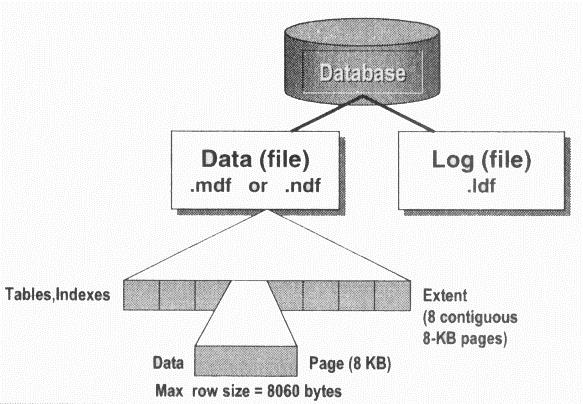
\includegraphics[width=.5\linewidth]{img/DatabaseCreatie.png}
  	\caption{Opbouw van een database}
  	\label{fig:DatabaseCreatie}
\end{figure}

Logfiles bevatten informatie nodig voor recovery.
De logfile-grootte is per default 25\% van grootte van de datafile.

In sql creëert men een database als volgt:
\begin{lstlisting}[language=sql]
CREATE DATABASE database_name
\end{lstlisting}

Men kan hierbij ook parameters meegeven:
\begin{lstlisting}[language=sql, breaklines=true]
CREATE DATABASE oefenDB 
ON PRIMARY(
	NAME = oefenDB_data,
	FILENAME = 'C:\Program Files\Microsoft SQL Server\ MSSQL.1\MSSQL\Data\oefenDB.mdf',
	SIZE = 10MB, MAXSIZE = 15MB, FILEGROWTH = 20%)
LOG ON (
	NAME = tttoefenDB_log,
	FILENAME = 'C:\Program Files\Microsoft SQL Server\ MSSQL.1\MSSQL\Data\oefenDB.ldf',
	SIZE = 3MB, MAXSIZE = 5MB, FILEGROWTH = 1MB)
\end{lstlisting}

\subsubsection{Een database verwijderen}
\begin{lstlisting}[language=sql, breaklines=true]
DROP DATABASE database_name
\end{lstlisting}

Hierbij dient opgemerkt te worden dat de systeem databank niet verwijderd kan worden.

\subsubsection{Een database wijzigen}
\begin{itemize}
\item beheer van de groei van de database en log file
\item uitbreiden/verminderen van grootte van database en log
\item toevoegen/verwijderen van secondary database files, log files
\end{itemize}

Wijzigen van de groote van het logbestand:
\begin{lstlisting}[language=sql, breaklines=true]
ALTER DATABASE oefenDB
MODIFY FILE (name = 'oefenDB_log', size = 10MB)
\end{lstlisting}

Toevoegen van een databastand:
\begin{lstlisting}[language=sql, breaklines=true]
ALTER DATABASE oefenDB
ADD FILE (
	name = oefenDB2,
	filename = 'C:\Program Files\Microsoft SQL Server\ MSSQL.1\MSSQL\Data\oefenDB2.ndf',
	size = 10MB,
	maxsize = 15MB)
\end{lstlisting}

\subsection{Tabellen}
\subsubsection{Een tabel creëren}
Bij de creatie van een tabel specifieren we:
\begin{itemize}
\item de naam van de tabel.
\item de definitie van de kolommen (naam, datatype \dots).
\item definitie van de constraints.
\end{itemize}

\begin{lstlisting}[language=sql, breaklines=true]
CREATE TABLE student(
	studentno int NOT NULL,
	lastname varchar(30) NOT NULL,
	firstname varchar(30) NOT NULL,
	gender char(1) NOT NULL,
	photograph image NULL)
\end{lstlisting}

\subsubsection{Een tabel wijzigen}
Mogelijke wijzigingen aan een tabel omvatten:
\begin{itemize}
\item toevoegen van kolommen.
\item wijzigen van kolommen.
\item verwijderen van kolommen.
\end{itemize}

\begin{lstlisting}[language=sql, breaklines=true]
ALTER TABLE student(
	ADD address varchar(40) NULL,
	ALTER COLUMN address varchar(50) NULL,
	DROP COLUMN address)
\end{lstlisting}

\subsubsection{Een tabel verwijderen}
Bij het verwijderen van een tabel diet men rekening te houden met de afhankelijkheden.

\begin{lstlisting}[language=sql, breaklines=true]
DROP TABLE student
\end{lstlisting}

\subsection{Contraints}
\subsubsection{Identity waarden}
Een identity kolom bevat voor elke rij een unieke waarde, die sequentieel door het systeem gegenereerd wordt.
Er is slechts één identity kolom per tabel mogelijk.
De identity kolom kan niet NULL zijn en kan niet door gebruikers aangepast worden.

\begin{lstlisting}[language=sql, breaklines=true]
CREATE TABLE studentVoorbeeldIdentity(
	studentno int identity(100, 5) NOT NULL,
	lastname varchar(30) NOT NULL,
	firstname varchar(30) NOT NULL,
	gender char(1) NOT NULL,
	photograph image NULL)
\end{lstlisting}

\subsubsection{Data integriteit}
Soorten:
\begin{itemize}
\item domein integriteit
\item entity integriteit
\item referentiële integriteit
\end{itemize}

\subsubsection{Definitie van constraints}
Via create table en als onderdeel van de kolomdefinitie:
\begin{lstlisting}[language=sql, breaklines=true]
CREATE TABLE studentVoorbeeldIdentity(
	studentno int NOT NULL unique)
\end{lstlisting}

Via alter table en als aparte lijn:
\begin{lstlisting}[language=sql, breaklines=true]
ALTER TABLE studentVoorbeeldIdentity(
	CONSTRAINT studentno_U unique(studentno)
\end{lstlisting}

Zowel bij creatie al bij wijzigen kan gekozen worden voor onderdeel van de kolomdefinitie als voor aparte lijn.
NULL en DEFAULT constraints kunnen enkel bij definitie van de kolom worden opgegeven.

\subsubsection{Check constraint}
\begin{lstlisting}[language=sql, breaklines=true]
gender char(1) default 'M' check(gender in ('M','F')) not null
\end{lstlisting}

\subsubsection{Primary key constraint}
\begin{lstlisting}[language=sql, breaklines=true]
studentno int primary key
\end{lstlisting}

of

\begin{lstlisting}[language=sql, breaklines=true]
constraint studentno_PK primary key(studentno)
\end{lstlisting}

\subsubsection{Foreign key constraint}
De foreign key wordt gebruikt om verbanden tussen relaties uit te drukken. NULL waarden zijn niet toegelaten.
\begin{lstlisting}[language=sql, breaklines=true]
constraint class_fk foreign key(class) references class(classID)
\end{lstlisting}
De foreign key legt ook de trapsgewijze (cascading) referentiële integriteitsacties vast.

\subsection{Views}
\subsubsection{Introductie}
Een view is een SELECT statement die onder een eigen naam wordt bewaard.
Een view is bijgevolg een soort virtuele tabel samengesteld uit andere tabellen of views.

De voordelen hiervan zijn dat de complexiteit van de database verborgen is.
Gebruikers krijgen functionaliteit en rechten op maat.
Views vereenvoudigen de beveiliging van de database.
Data wordt ook georganiseerd voor de export naar andere applicaties.

\begin{lstlisting}[language=sql, breaklines=true]
CREATE VIEW view_name [(column_list)]
AS select_statement
\end{lstlisting}

Views kunnen net als tabellen verwijders en gewijzigd worden.
\end{document}